\section{Конструкторская часть}
    \par В данном разделе разрабатывается метод воспроизведения потокового \newline аудио 
    в мобильном приложении на операционной системе iOS.
    Выделяются основные компоненты разрабатываемого программно-алгоритмического комплекса, 
    а также описывается их взаимодействие между собою. 
    Основные алгоритмы представлены в виде схем.

    \subsection{Формализация задачи}
        \subsubsection{Требования к разрабатываемому методу}
            \par Метод воспроизведения потокового аудио в мобильном приложении на операционной системе iOS,
            который будет использован в разрабатываемом программном комплексе, 
            должен удовлетворять следующим требованиям:
            \begin{itemize}
                \item[---] на вход принимается поток пакетов аудиоданных, отправляемых стороной сервера по протоколу HTTP;
                \item[---] приходящие аудиоданные должны обрабатываться в PCM формате;
                \item[---] приходящие аудиоданные должны содержать метаинформацию (заголовок) воспроизводимого файла;
                \item[---] для наложения звуковых эффектов строится дерево аудиоузлов, задающих правила обработки звукового сигнала;
            \end{itemize}

        \subsubsection{IDEF0–диаграмма}
            \par На рис. \ref{fig:idef0} и \ref{fig:idef0-det} представлены 
            диаграмма IDEF0 метода воспроизведения потокового аудио в мобильном приложении,
            а также декомпозиция диаграммы IDEF0 на подзадачи A1-A4 соответственно. 
            Описание декомпозированных задач рассмотрено ниже.

            \newpage
            \begin{figure}[!h]
                \center{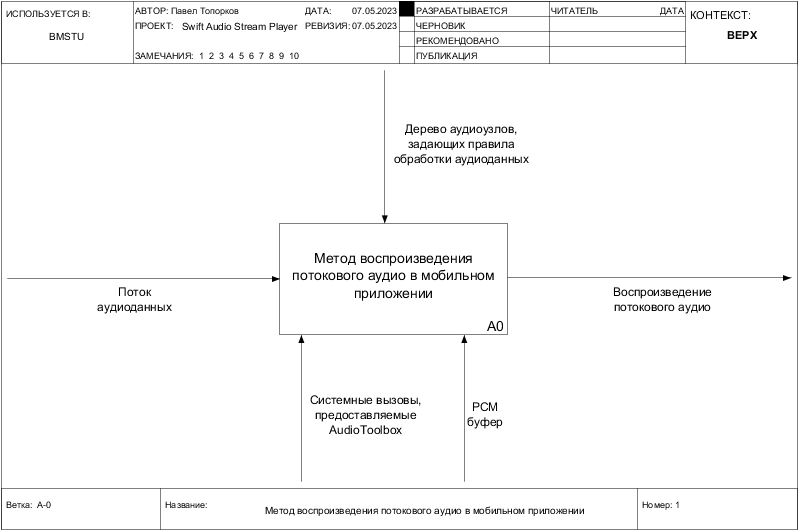
\includegraphics[scale=0.52]{img/01_A-0.png}}
                \caption{Диграмма IDEF0 метода воспроизведения потокового аудио в мобильном приложении.}
                \label{fig:idef0}
            \end{figure}

            \begin{figure}[!h]
                \center{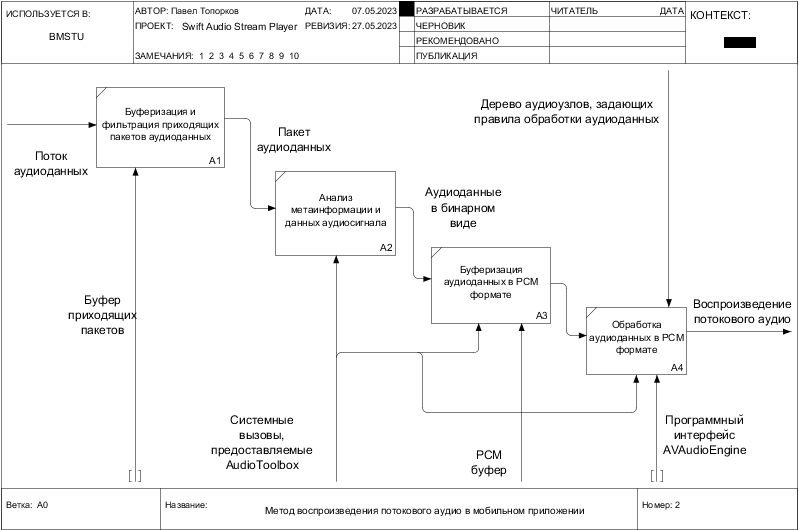
\includegraphics[scale=0.52]{img/02_A0.png}}
                \caption{Декомпозиция диграммы IDEF0 на подзадачи A1-A4.}
                \label{fig:idef0-det}
            \end{figure}
    
    \subsection{Буферизация и фильтрация приходящих пакетов данных}
        \par Для контроля нагрузки ЦПУ мобильного устройства необходимо ограничивать запрос потока аудиоданных.
        Выделяется специальный механизм буферизации приходящих пакетов данных, 
        а также фильтруется подача аудиоданных обработчику данных.
        В момент переполнения буфера приходящих пакетов прекращается запрос новых данных, 
        пока в буфере не освободится место. 
        Данное решение продиктовано тем, 
        что при использовании сетевых запросов мобильное устройство интенсивнее использует вычислительные мощности ЦПУ, 
        критическая нагрузка может доходить до $90-100\%$ при периодичном сетевом подключении \cite{CPUUtilization}.

        \par На рис. \ref{fig:throttler-scheme} представлена схема алгоритма буферизации и фильтрации приходящих пакетов данных.
        \begin{figure}[!h]
            \center{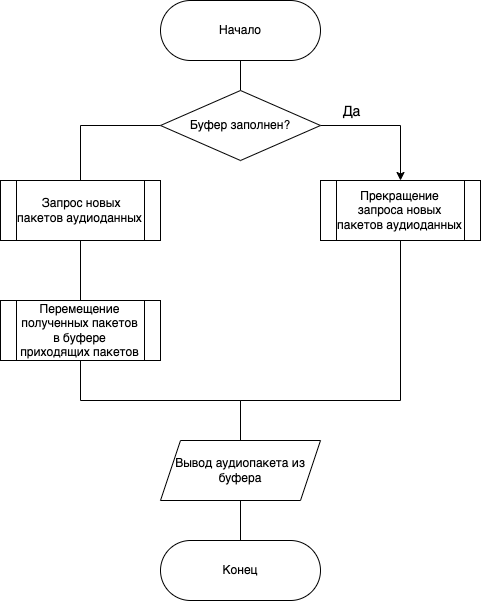
\includegraphics[scale=0.55]{img/throttler-scheme.png}}
            \caption{Cхема алгоритма буферизации и фильтрации приходящих пакетов данных.}
            \label{fig:throttler-scheme}
        \end{figure}

    \subsection{Анализ информации и данных аудиосигнала}
        \par Поступаемые аудиоданные необходимо проанализировать, 
        чтобы определить формат оригинального аудиофайла, 
        метаинформацию и данные, содержащие информацию о воспроизведении аудиосигнала.

        \par Для обработки информации об аудиосигнале необходимо определить формат файла.
        Формат должен содержаться в метаинформации аудиофайла, которая передаётся в первых пришедших пакетах данных.
        Также необходимо определить частоту дискретизации аудиосигнала и количество фреймов в пакете.
        На рис. \ref{fig:parser-analys} представлена схема анализа информации и данных аудиосигнала.
        \begin{figure}[!h]
            \center{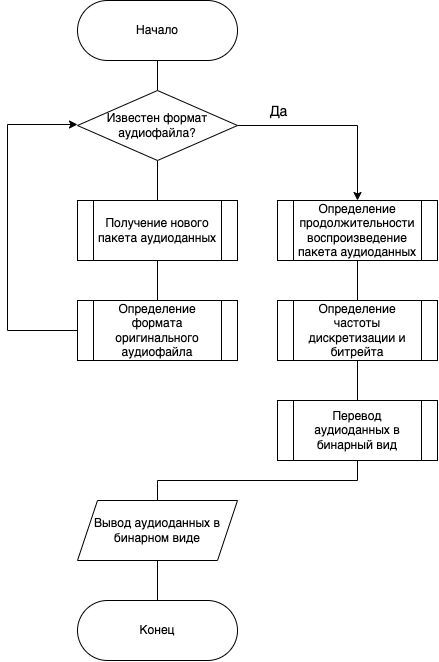
\includegraphics[scale=0.65]{img/parser-analys.png}}
            \caption{Схема анализа информации и данных аудиосигнала.}
            \label{fig:parser-analys}
        \end{figure}

        \par Для получения информации о звуковом сигнале необходимо из получаемого пакета аудиоданных отделить 
        метаинформацию, а также заголовки сегментов от данных аудиосигнала. 
        На рис. \ref{fig:audiofile-line} представлены линейные представления аудиофайла,
        а также сегмента (фрейма) аудиоданных файла с расположением метаданных, заголовков и данных аудиосигнала.
        
        \begin{figure}[!h]
            \center{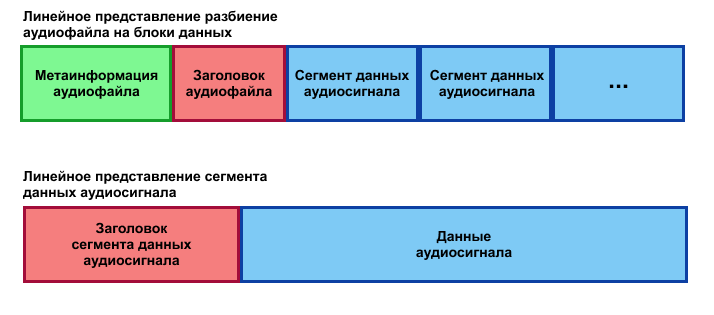
\includegraphics[scale=0.65]{img/audiofile-line.png}}
            \caption{Линейные представления аудиофайла, а также сегмента (фрейма) аудиоданных файла.}
            \label{fig:audiofile-line}
        \end{figure}

        \par Важной информацией для обработки аудио является продолжительность воспроизведения аудио, 
        полученного из пришедшего пакета данных.
        Некоторые аудиофайлы могут не содержать продолжительность воспроизведения в своих метаданных. 
        В таком случае необходимо определить продолжительность сигнала в аудиопакете самостоятельно с учётом возможного переменного битрейта.
        Продолжительность воспроизведения можно получить по формуле:
        $$ t = \frac{b}{f},$$
        где
        \begin{itemize}
            \item[] $t$ --- продолжительность воспроизведения;
            \item[] $n$ --- количество фреймов в пакете аудиоданных;
            \item[] $f$ --- частота дискретизации.
        \end{itemize}

    \subsection{Буферизация аудиоданных в PCM формате}
        \par Аудиоданные в бинарном виде, полученные с помощью анализа данных аудиосигнала, буферизуются в PCM формате.
        Для этого создаётся специальный, системный PCM буфер, который хранит фреймы аудиоданных, 
        предназначенных для текущего воспроизведения. 
        После заполнения PCM буфера необходимо воспользоваться системными вызовами для воспроизведения аудиосигнала.
        Размер PCM буфера определяется в зависимости от разрешения звука.
        Ниже указано количество фреймов аудиоданных, содержащихся в PCM буфере в зависимости от разрешения звука:
        \begin{itemize}
            \item[---] для низкого разрешения звука --- 4096 фреймов;
            \item[---] для высокого разрешения звука --- 8192 фрейма;
        \end{itemize}

        \par На рис. \ref{fig:schema-pcm-buff} представлена схема буферизации аудиоданных в PCM формате.
        \begin{figure}[!h]
            \center{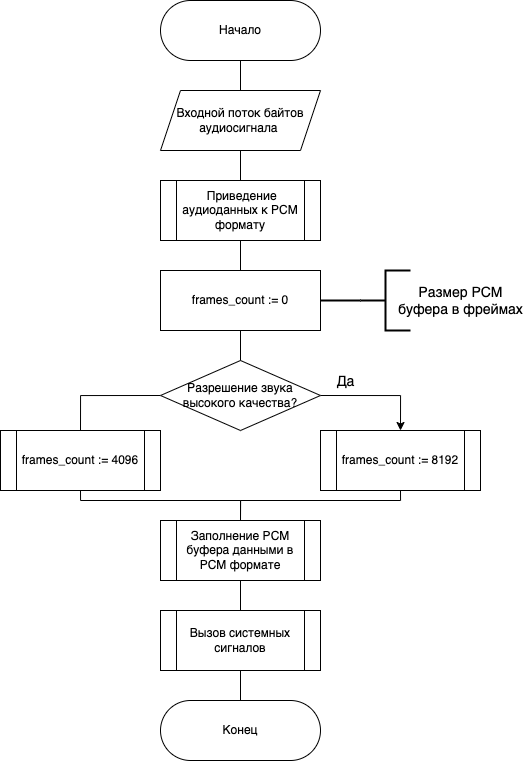
\includegraphics[scale=0.42]{img/schema-pcm-buff.png}}
            \caption{Схема буферизации аудиоданных в PCM формате.}
            \label{fig:schema-pcm-buff}
        \end{figure}

    \subsection{Обработка аудиоданных в PCM формате}
        \par После помещения аудиоданных в PCM буфер необходимо начать процесс воспроизведения аудиоданных.
        Для этого с помощью системного вызова \newline AudioFileStreamOpen нужно инициировать процесс анализа аудиоданных.
        
        \par Также необходимо создать дерево аудиоузлов обработки аудиосигнала, которые наложат звуковые эффекты на воспроизводимый аудиосигнал.
        При старте воспроизведения нужно связать программный интерфейс AVAudioEngine с построенным деревом аудиоузлов.
        AVAudioEngine становится частью дерева аудиоузлов обработки, отвечая за определения характеристик музыкального сигнала.
        В случае ошибки обработки аудиосигнала вызовется системное прерывание.

        \par На рис. \ref{fig:handler-pcm-format} представлена схема обработки аудиоданных в PCM формате.
        \begin{figure}[!h]
            \center{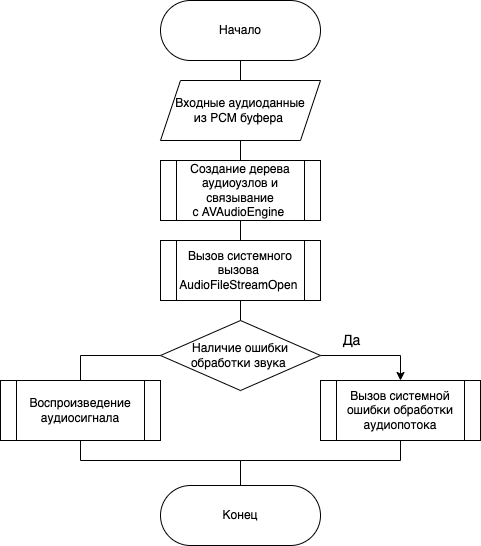
\includegraphics[scale=0.63]{img/handler-pcm-format.png}}
            \caption{Cхема обработки аудиоданных в PCM формате.}
            \label{fig:handler-pcm-format}
        \end{figure}

    \subsection{Основные компоненты разрабатываемого программного комплекса}
        \par Из вышеизложенного следует, 
        что к основным компонентам разрабатываемого программно-алгоритмического 
        комплекса необходимо отнести следующие:
        \begin{itemize}
            \item[---] компонент сетевых запросов;
            \item[---] компонент управления потоком данных;
            \item[---] компонент обработки пакетов;
            \item[---] компонент конвертации пакетов аудиоданных;
            \item[---] компонент воспроизведения аудиоданных;
        \end{itemize}

        % \subsubsection{Компонент сетевых запросов}
            \par Компонент сетевых запросов отвечает за получение новых пакетов аудиоданных со стороны сервера.
            Он определяет заголовки запросов данных, устанавливает HTTP соединение.
            
            \par Сетевой компонент получает данные в чистом (бинарном) виде, поддерживая постоянное соединение с сервером для
            быстрого получения новых пакетов аудиоданных при необходимости. При приостановке или разрыве соединения, 
            данный компонет должен запомнить параметры, тип и статус соединения для его востановления при новом запросе аудиопакетов. 

        % \subsubsection{Компонент управления потоком данных}
            \par Компонент управления потоком данных получает данные от компонента сетевых запросов 
            и определяет необходимость запроса новых аудиопакетов. 
            
            \par С его помощью решается задача буферизации и фильтрации приходящих пакетов данных:
            построение буфера приходящих пакетов данных, контроль переполнения буфера, буферизация новых пакетов данных.
            Данный компонет можно рассматривать как пропускающий механизм пакетов, передаваемых
            компоненту обработки пакетов.
            
        % \subsubsection{Компонент обработки пакетов}
            \par Компонент обработки пакетов решает задачу анализа информации и данных аудиосигнала.
            При получении сетевых данных выполняется анализ следующей находящейся в них информации:
            \begin{itemize}
                \item[---] метаинформация аудиофайла;
                \item[---] заголовок аудиофайла;
                \item[---] сегменты аудиосигнала;
                \item[---] заголовки сегментов аудиосигнала;
                \item[---] данные аудиосигнала, находящиеся в сегментах аудиофайла;
            \end{itemize}

            \par Главной задачей данного компонента является получение данных аудиосигнала, 
            а также выявление метаинформации для корректного воспроизведения аудиосигнала.

        % \subsubsection{Компонент конвертации пакетов аудиоданных}
            \par Обработанные пакеты необходимо конвертировать в формат, подходящий для воспроизведения аудиосигнала.
            На основе полученных метаинформации и формата определяется размер создаваемого PCM буфера 
            и происходит его заполнение данными аудиосигнала. 
            Полученная метаинформация позволяет сообщить системе о характеристиках звукового сигнала, 
            продолжительности воспроизведения, а также обработать информацию для управления потоком воспроизведения.
            Следует отметить, что компонент конвертации пакетов аудиоданных решает задачу буферизации аудиоданных в PCM формате.
        
        % \subsubsection{Компонент воспроизведения аудиоданных}
            \par Компонент воспроизведения аудиоданных решает задачу обработки аудиоданных в PCM формате.
            С помощью созданного дерева аудиоузлов, предназначенных для наложения звуковых эффектов, 
            а также AVAudioEngine происходит настройка системы для начала воспроизведения аудиосигнала.
            Для анализа аудиоданных, предназначенных для воспроизведения с помощью \newline AVAudioEngine, 
            необходимо воспользоваться системными вызовами.

        \subsubsection{Взаимодействие компонентов разрабатываемого программного комплекса}
            \par Компоненты разрабатываемого программно-алгоритмического комплекса должны взаимодействовать по следующим правилам:
            \begin{itemize}
                \item[---] компонент сетевых запросов адресует полученные аудиопакеты компоненту управления потоком данных, 
                если буфер приходящих пакетов данных не переполнен;
                \item[---] компонент управления потоком отправляет буферизированные пакеты \newline компоненту обработки пакетов;
                \item[---] компонент конвертации пакетов аудиоданных запрашивает информацию из обработанных компонентом обработки пакетов сетевых данных;
                \item[---] компонент воспроизведения аудиоданных запрашивает конвертированные аудиоданные из компонента конвертации пакетов;
            \end{itemize}

            \par На рис. \ref{fig:audio-components} представлена схема взаимодействия компонентов.
            \begin{figure}[!h]
                \center{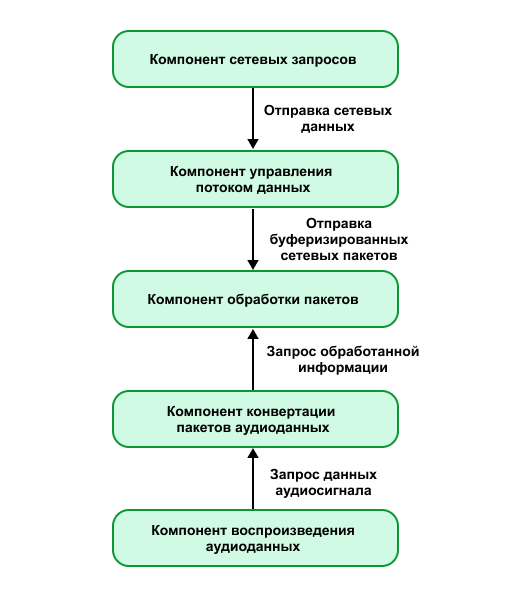
\includegraphics[scale=0.53]{img/audio-components.png}}
                \caption{Cхема взаимодействия компонентов.}
                \label{fig:audio-components}
            \end{figure}
        
    \subsection*{Вывод}
        \par В данном разделе был разработан метод воспроизведения потокового аудио в мобильном приложении на операционной системе iOS. 
        Были выделены основные компоненты разрабатываемого программно-алгоритмического комплекса, а также описано их взаимодействие между собою. 
        Приведены IDEF0 диаграмма, её декомпозиция, а также основные алгоритмы в виде схем.
\pagebreak